\chapter{Konzeption}

\section{Übersicht}

Zur Umsetzung des \textit{Smart Warehouse} Szenarios sind einige fundierte, konzeptionelle Überlegungen notwendig, die in diesem Kapitel betrachtet werden sollen. Sie beschränken sich auf sechs übergeordnete Themenbereiche, die in Abbildung \ref{schritte} dargestellt sind. 

\begin{figure}[H]
	\begin{center}
		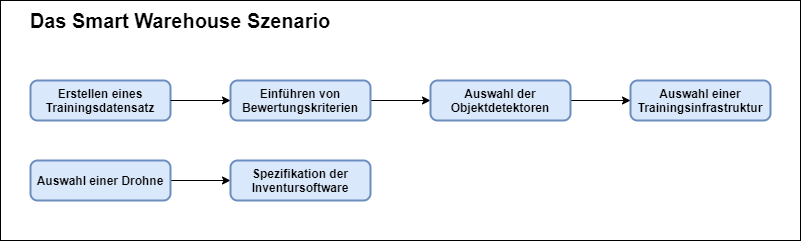
\includegraphics[width=15cm]{Bilder/blockdiagramm.png} 
		\caption[Konzeptionelle Schritte]{Konzeptionelle Schritte}
		\label{schritte}
	\end{center}
\end{figure}

Daraus ergeben sich zwei Neuheitswerte im Rahmen dieser Studienarbeit. Zum einen soll evaluiert werden, wie gut die bestehenden Objektdetektoren für industrielle Anwendungsszenarien grundsätzlich geeignet sind, zum anderen, ob das spezifische Anwendungsszenario zur Durchführung einer Inventur von Warenhäusern mit einer Drohne prototypisch umsetzbar ist.

Für das \textit{Smart Warehouse} Szenario ist demnach zum einen die Entwicklung eines \textit{Deep Learning} Modells notwendig, das auf das Anwendungsszenario einer Inventur von Warenhäusern spezialisiert ist. Hierzu muss ein geeigneter Trainingsdatensatz erstellt werden, auf dem die ausgewählten Objektdetektoren trainiert werden sollen. Um die Objektdetektoren miteinander vergleichen zu können, ist zudem die Einführung von Bewertungskriterien notwendig. Auf Basis dieser Kriterien wird später evaluiert, wie gut die ausgewählten Objektdetektoren sich allgemein für einen industriellen Einsatz eignen. Welche Objektdetektoren überhaupt im Sinne des \textit{Smart Warehouse} Szenarios miteinander verglichen werden sollen, ist im nächsten Schritt \glqq Auswahl der Objektdetektoren\grqq{} zu beschließen. Anschließend stellt sich nur noch die Frage, auf welcher Infrastruktur die Objektdetektoren trainiert werden sollen.

Um das zweite Ziel der Arbeit zu erarbeiten, kann auf den Ergebnissen des ersten Ziels aufgebaut werden. Eine Drohne soll die benötigten Daten zur Inferenz liefern. Welche Drohne dies sein soll, ist im ersten Schritt zu erarbeiten. Außerdem müssen die Daten der Drohne, hinsichtlich des Gedanken eine Inventur durchzuführen, passend verarbeitet und visualisiert werden. Diese \textit{Inventursoftware} ist im letzten Schritt in ihrem Umfang zu spezifizieren.

\section{Erstellen eines Trainingsdatensatzes} \label{traindata}

Das \textit{Smart Warehouse} lehnt sich an ein großes Warenhaus an, bei dem Produkte nicht in Kartons verpackt, sondern als ganzes auf Regalen angeordnet sind, ähnlich wie bei Warenhäusern wie \textit{Baumarkt} oder \textit{Selgros}. Bei dem Aufbau des Trainingsdatensatzes hat die Machbarkeitsstudie allerdings nicht zum Ziel, ein solches Warenhaus vollständig im Datensatz abzubilden, sondern wesentlich den Datensatz so umfangreich zu wählen, um eine generelle Umsetzbarkeit des \textit{Smart Warehouse} Szenarios zu beweisen. Im Rahmen des Projektes wurde sich deshalb exemplarisch auf Getränkeflaschen eines Warenhauses konzentriert. Dabei wurden neun Kategorien festgelegt (siehe Abbildung \ref{categories}). 

\begin{figure}[H]
	\subfigure[Saskia Wasser Klein]{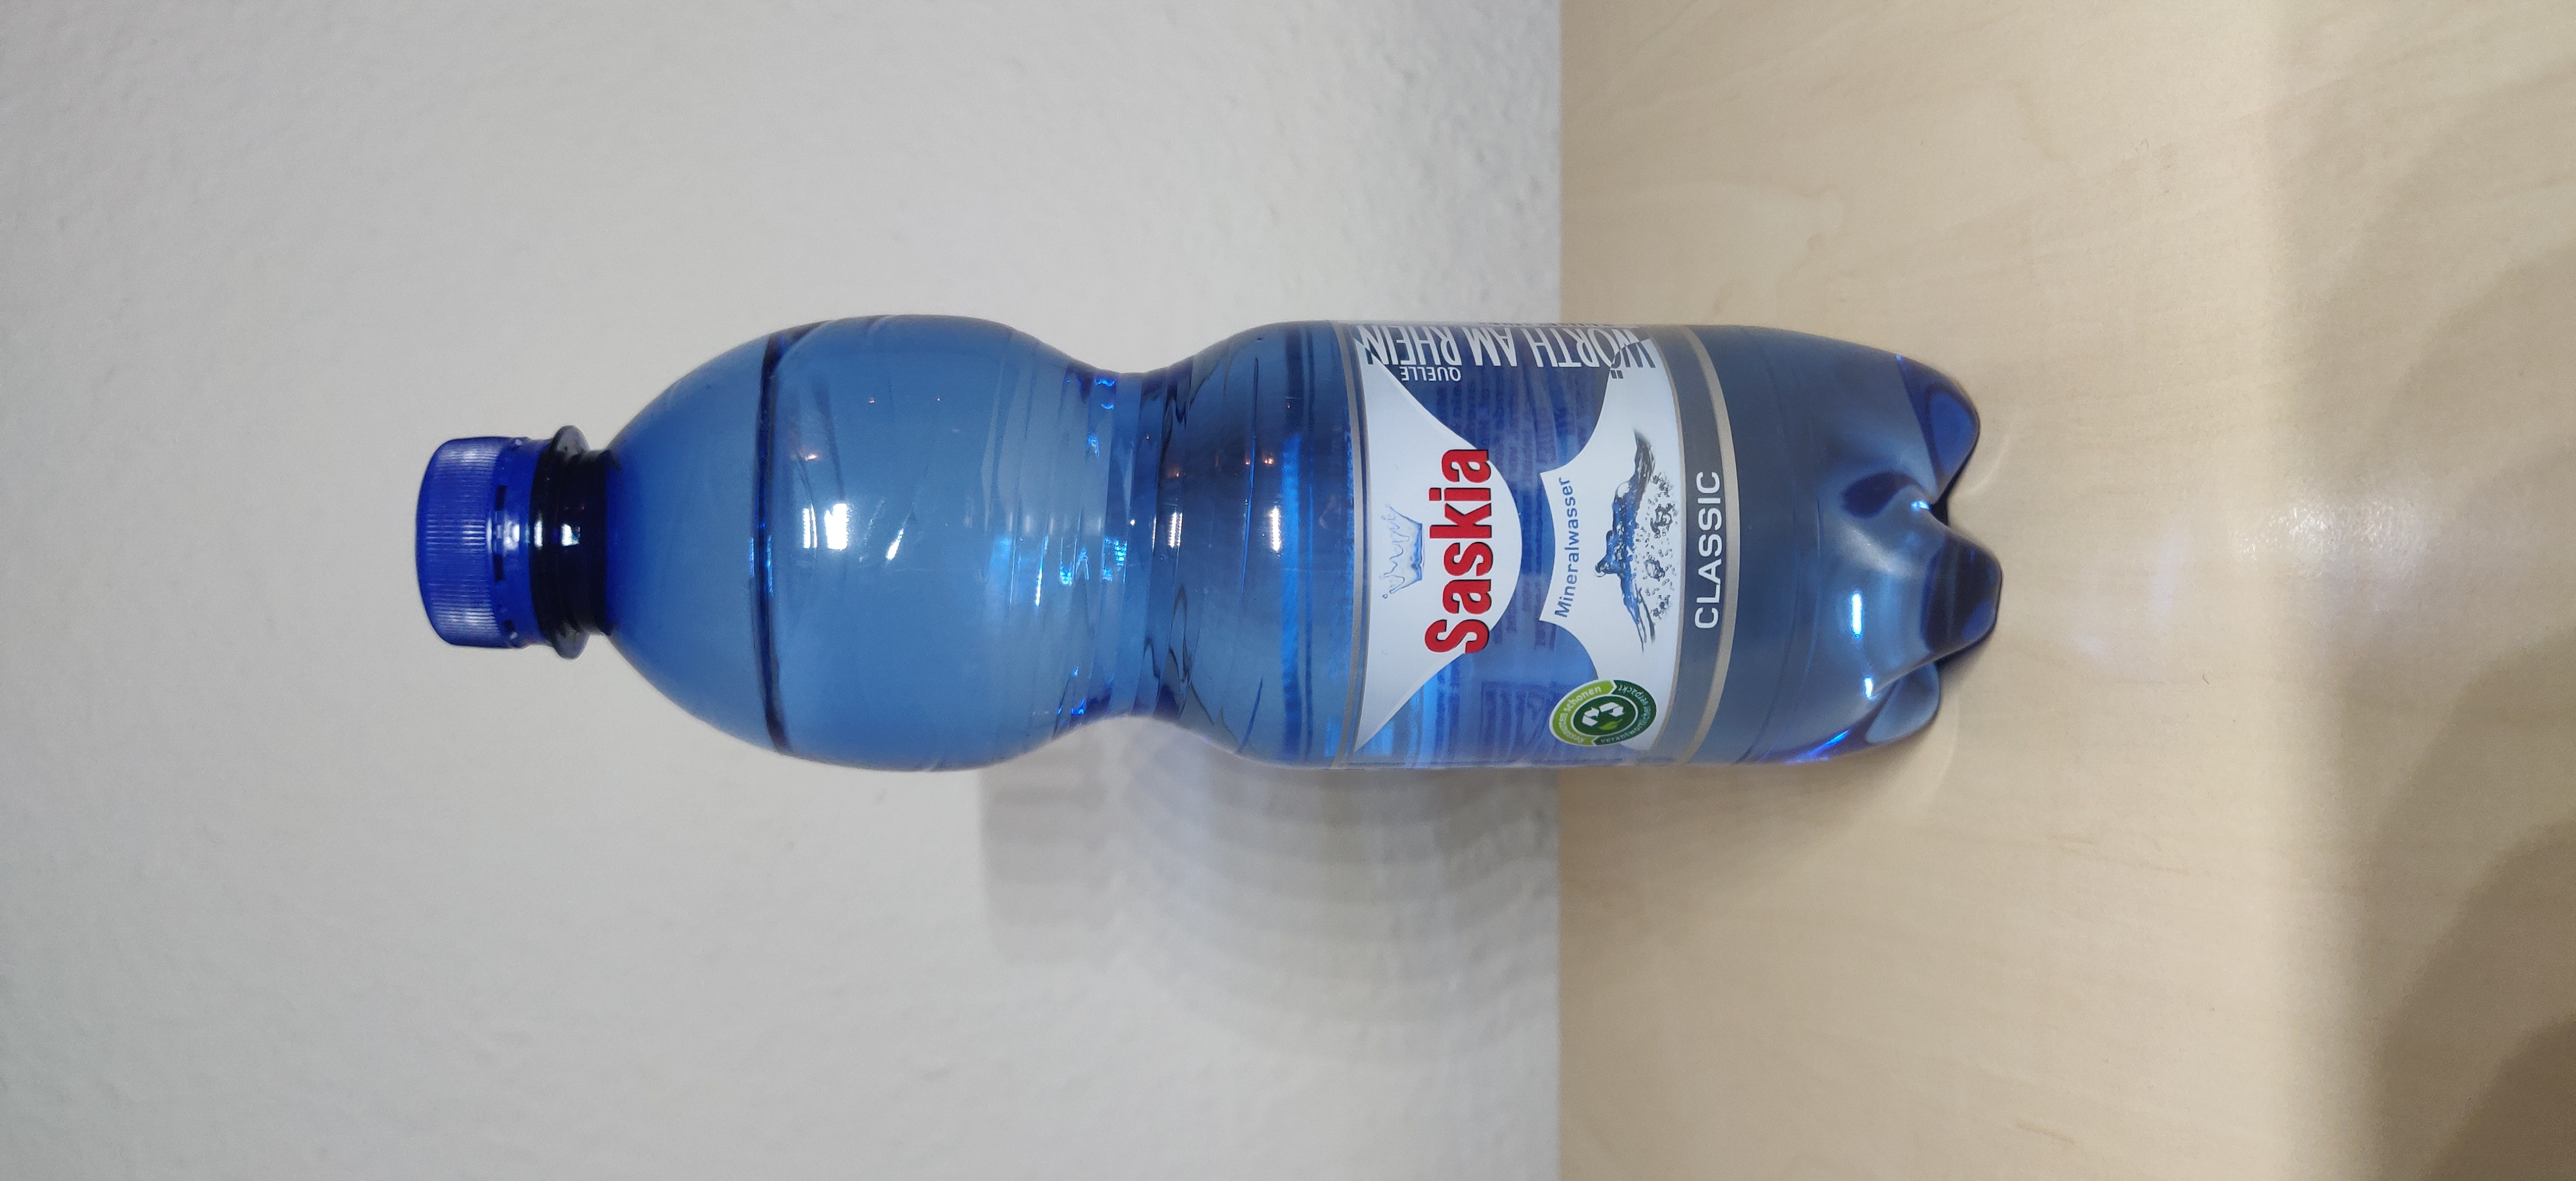
\includegraphics[width=0.30\textwidth]{Bilder/wasser_klein.jpg}}\hfill
	\subfigure[Saskia Wasser Groß]{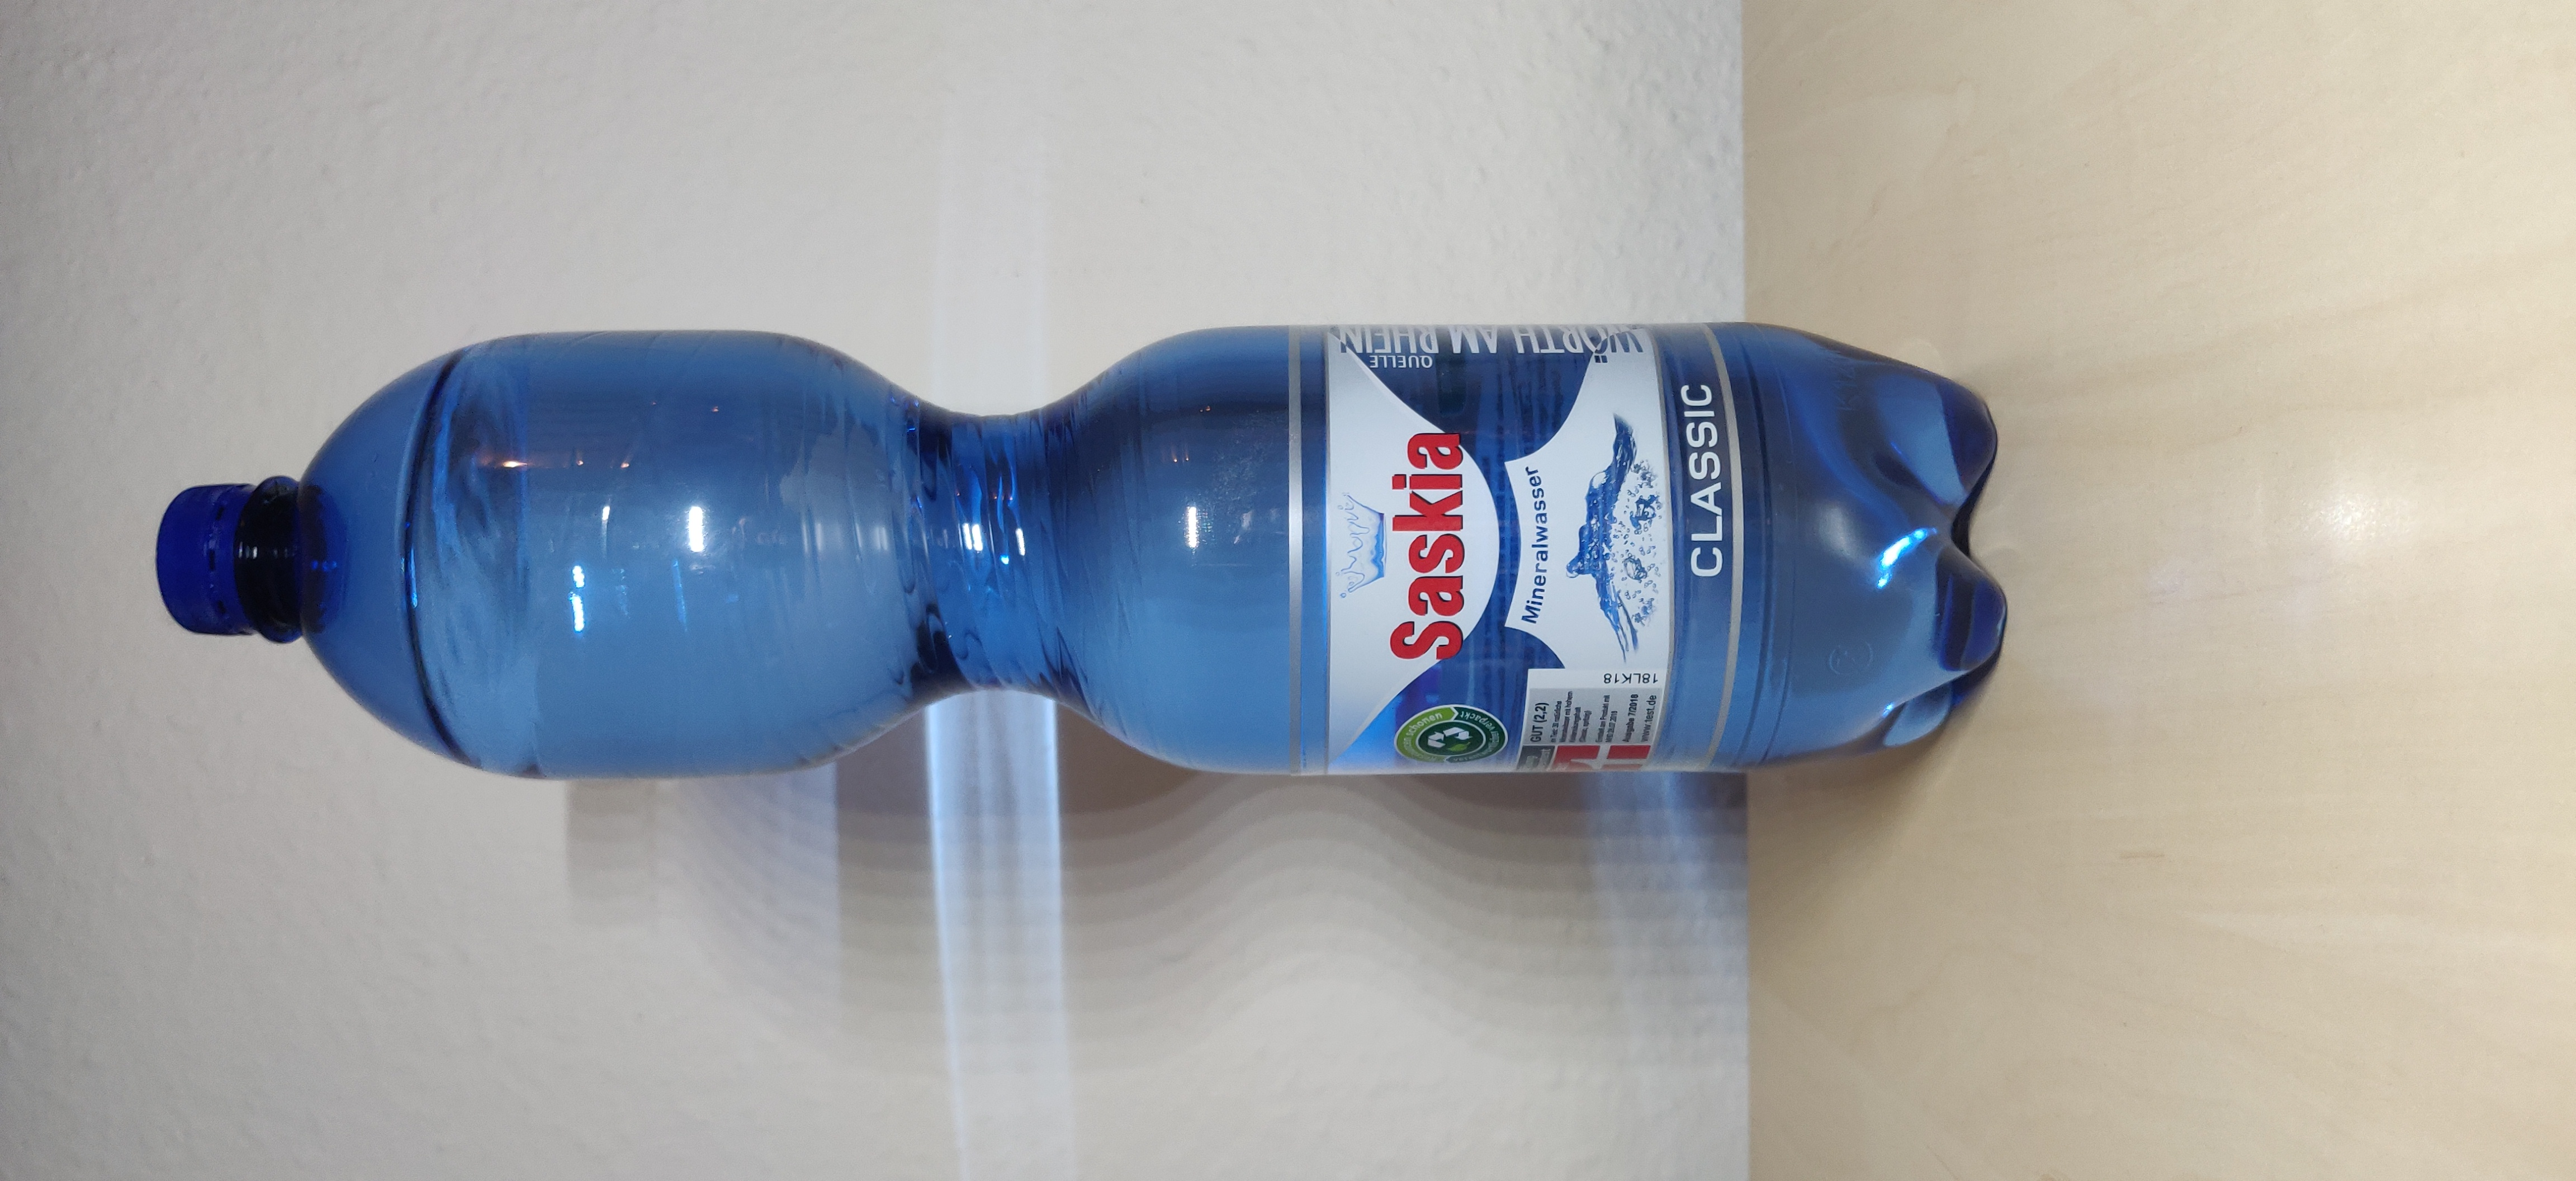
\includegraphics[width=0.30\textwidth]{Bilder/wasser_gross.jpg}}\hfill
	\subfigure[Pepsi Cola Klein]{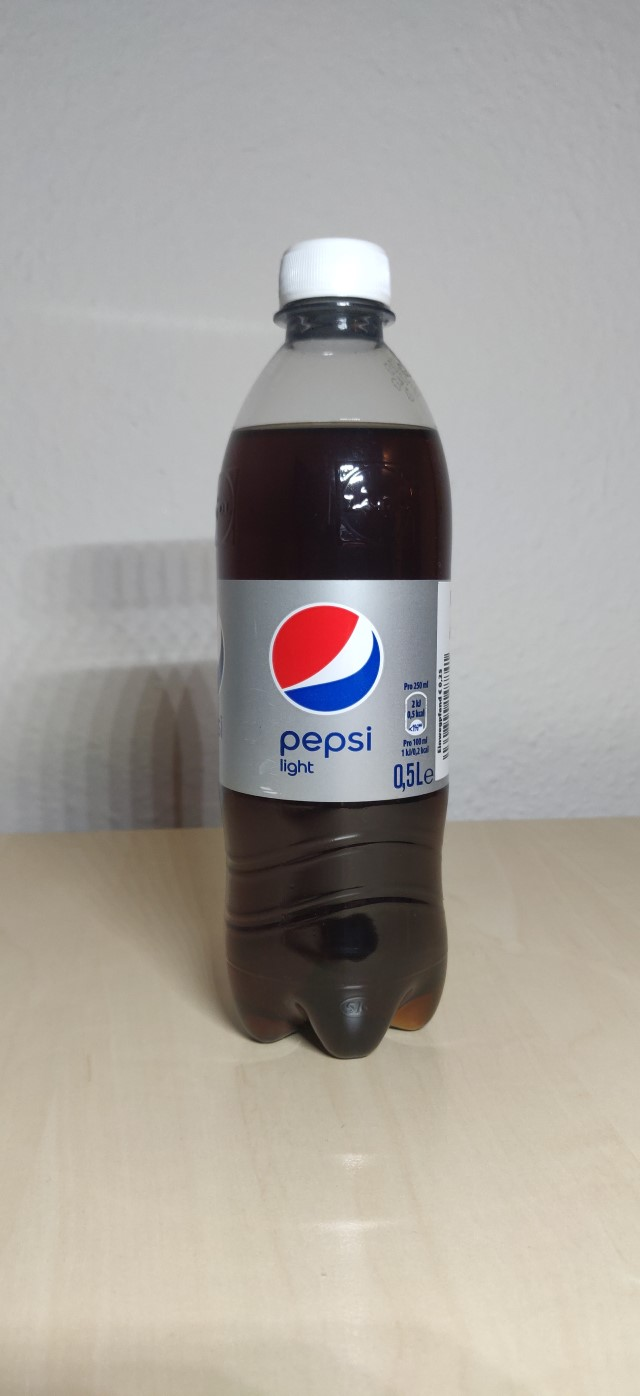
\includegraphics[width=0.30\textwidth]{Bilder/cola_klein.jpg}}\hfill
	\subfigure[Pepsi Cola Groß]{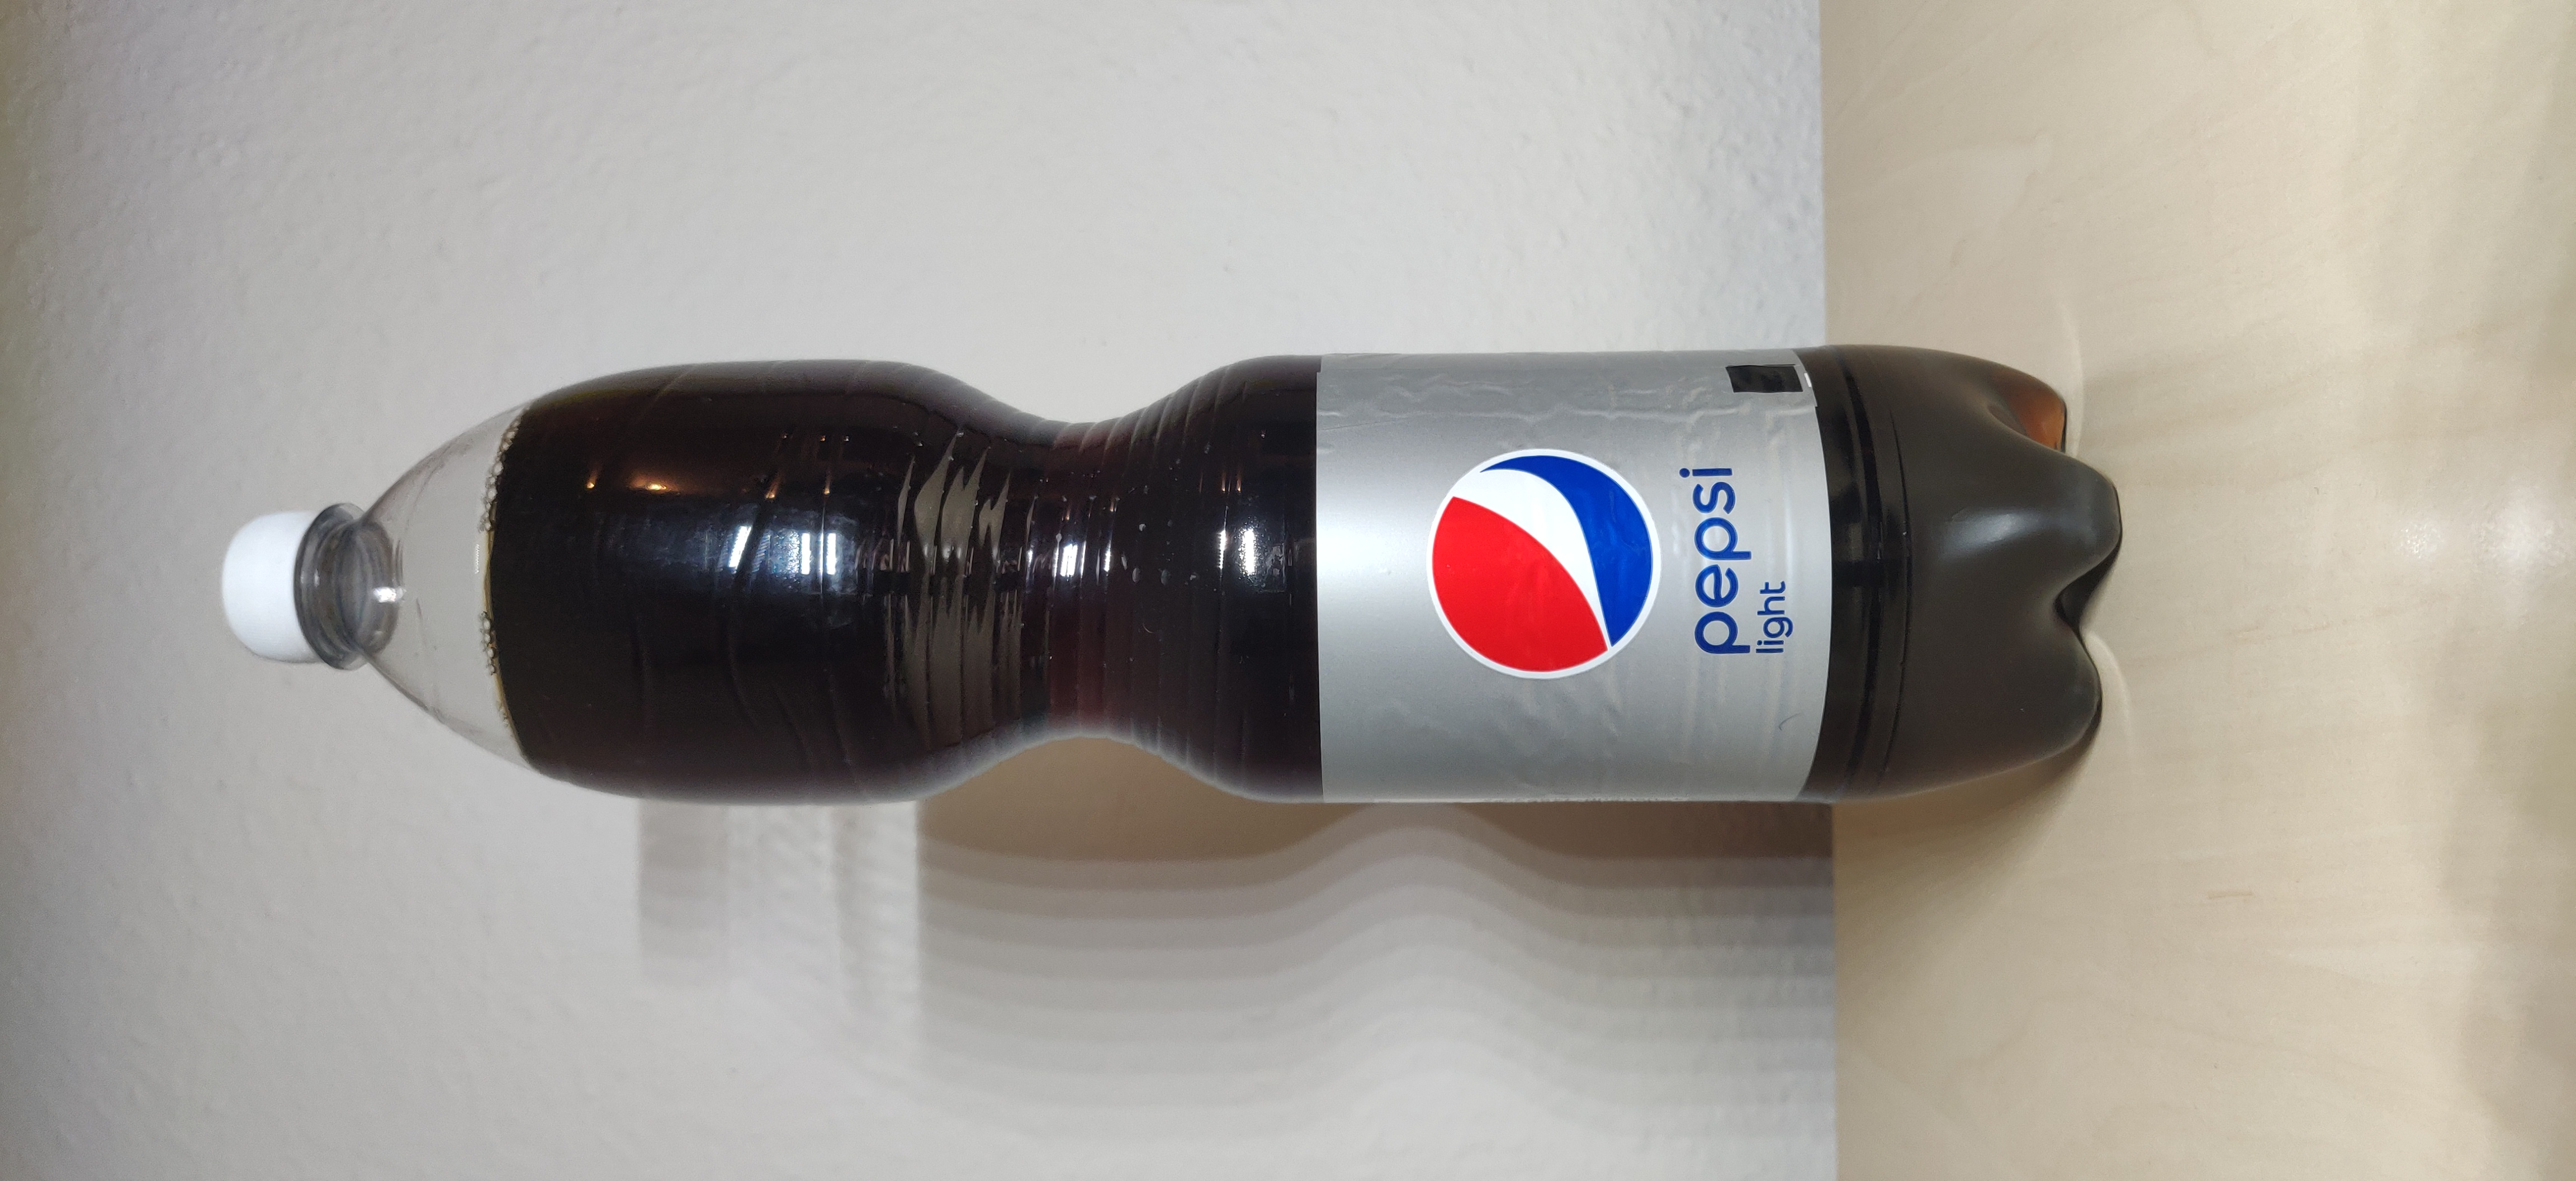
\includegraphics[width=0.30\textwidth]{Bilder/cola_gross.jpg}}\hfill
	\subfigure[ISO]{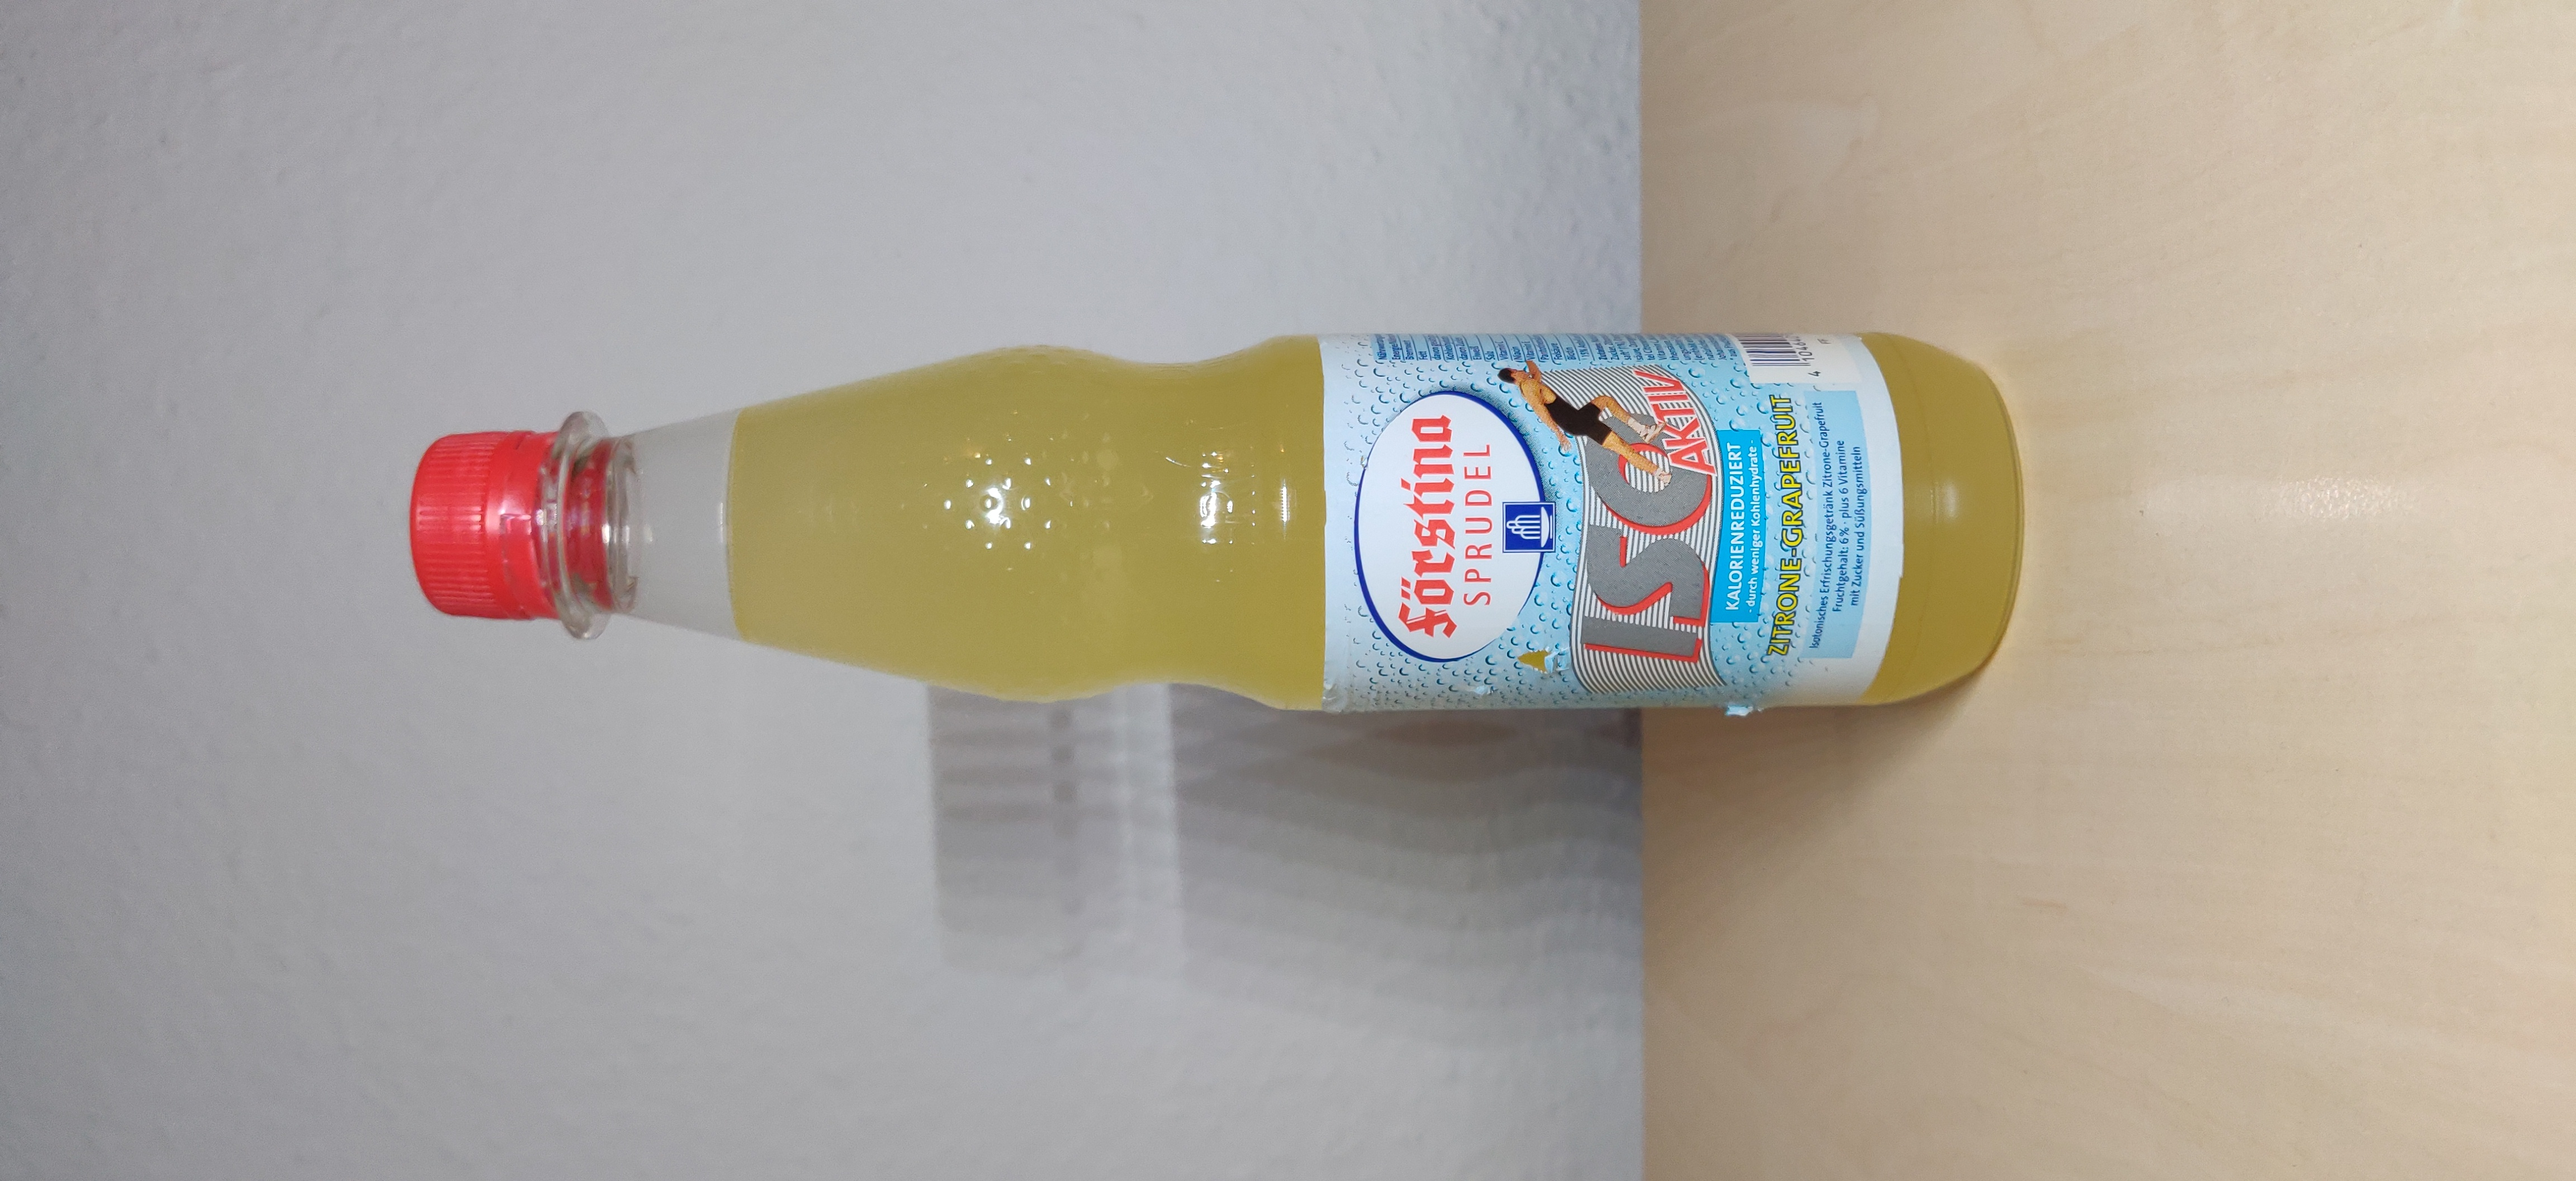
\includegraphics[width=0.30\textwidth]{Bilder/iso.jpg}}\hfill
	\subfigure[ACE]{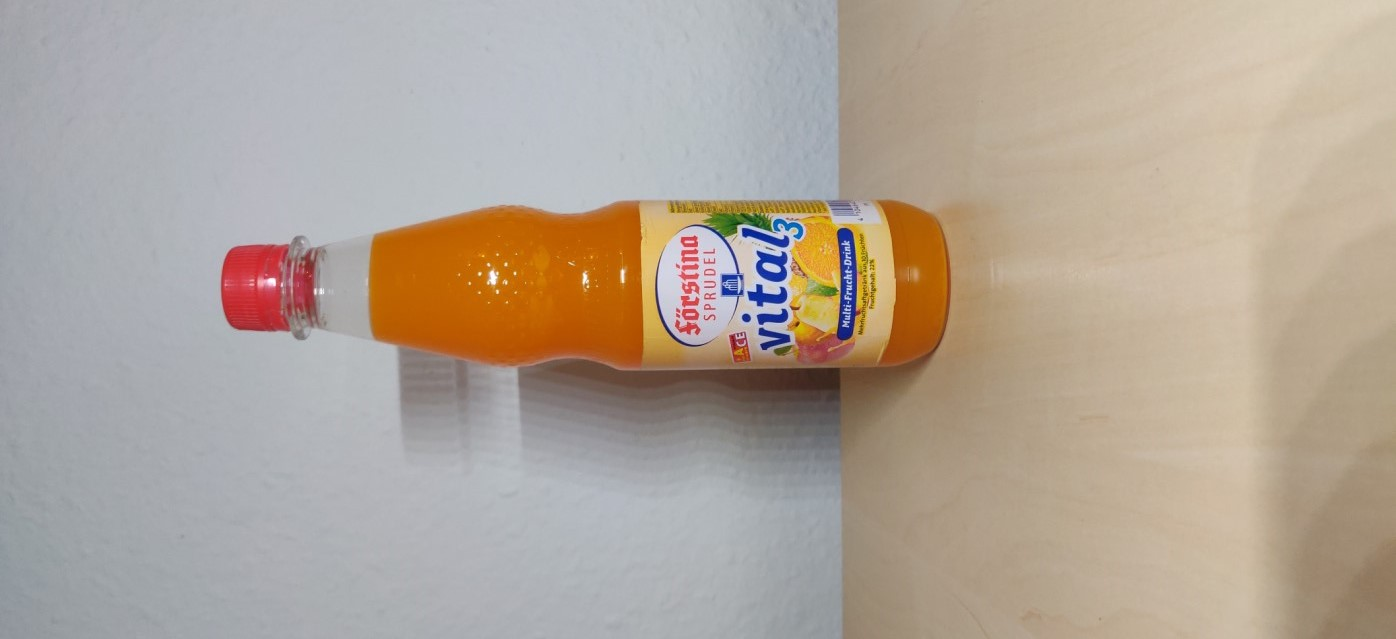
\includegraphics[width=0.30\textwidth]{Bilder/ace.jpg}}\hfill
	\subfigure[Stenger Johannisbeerschorle]{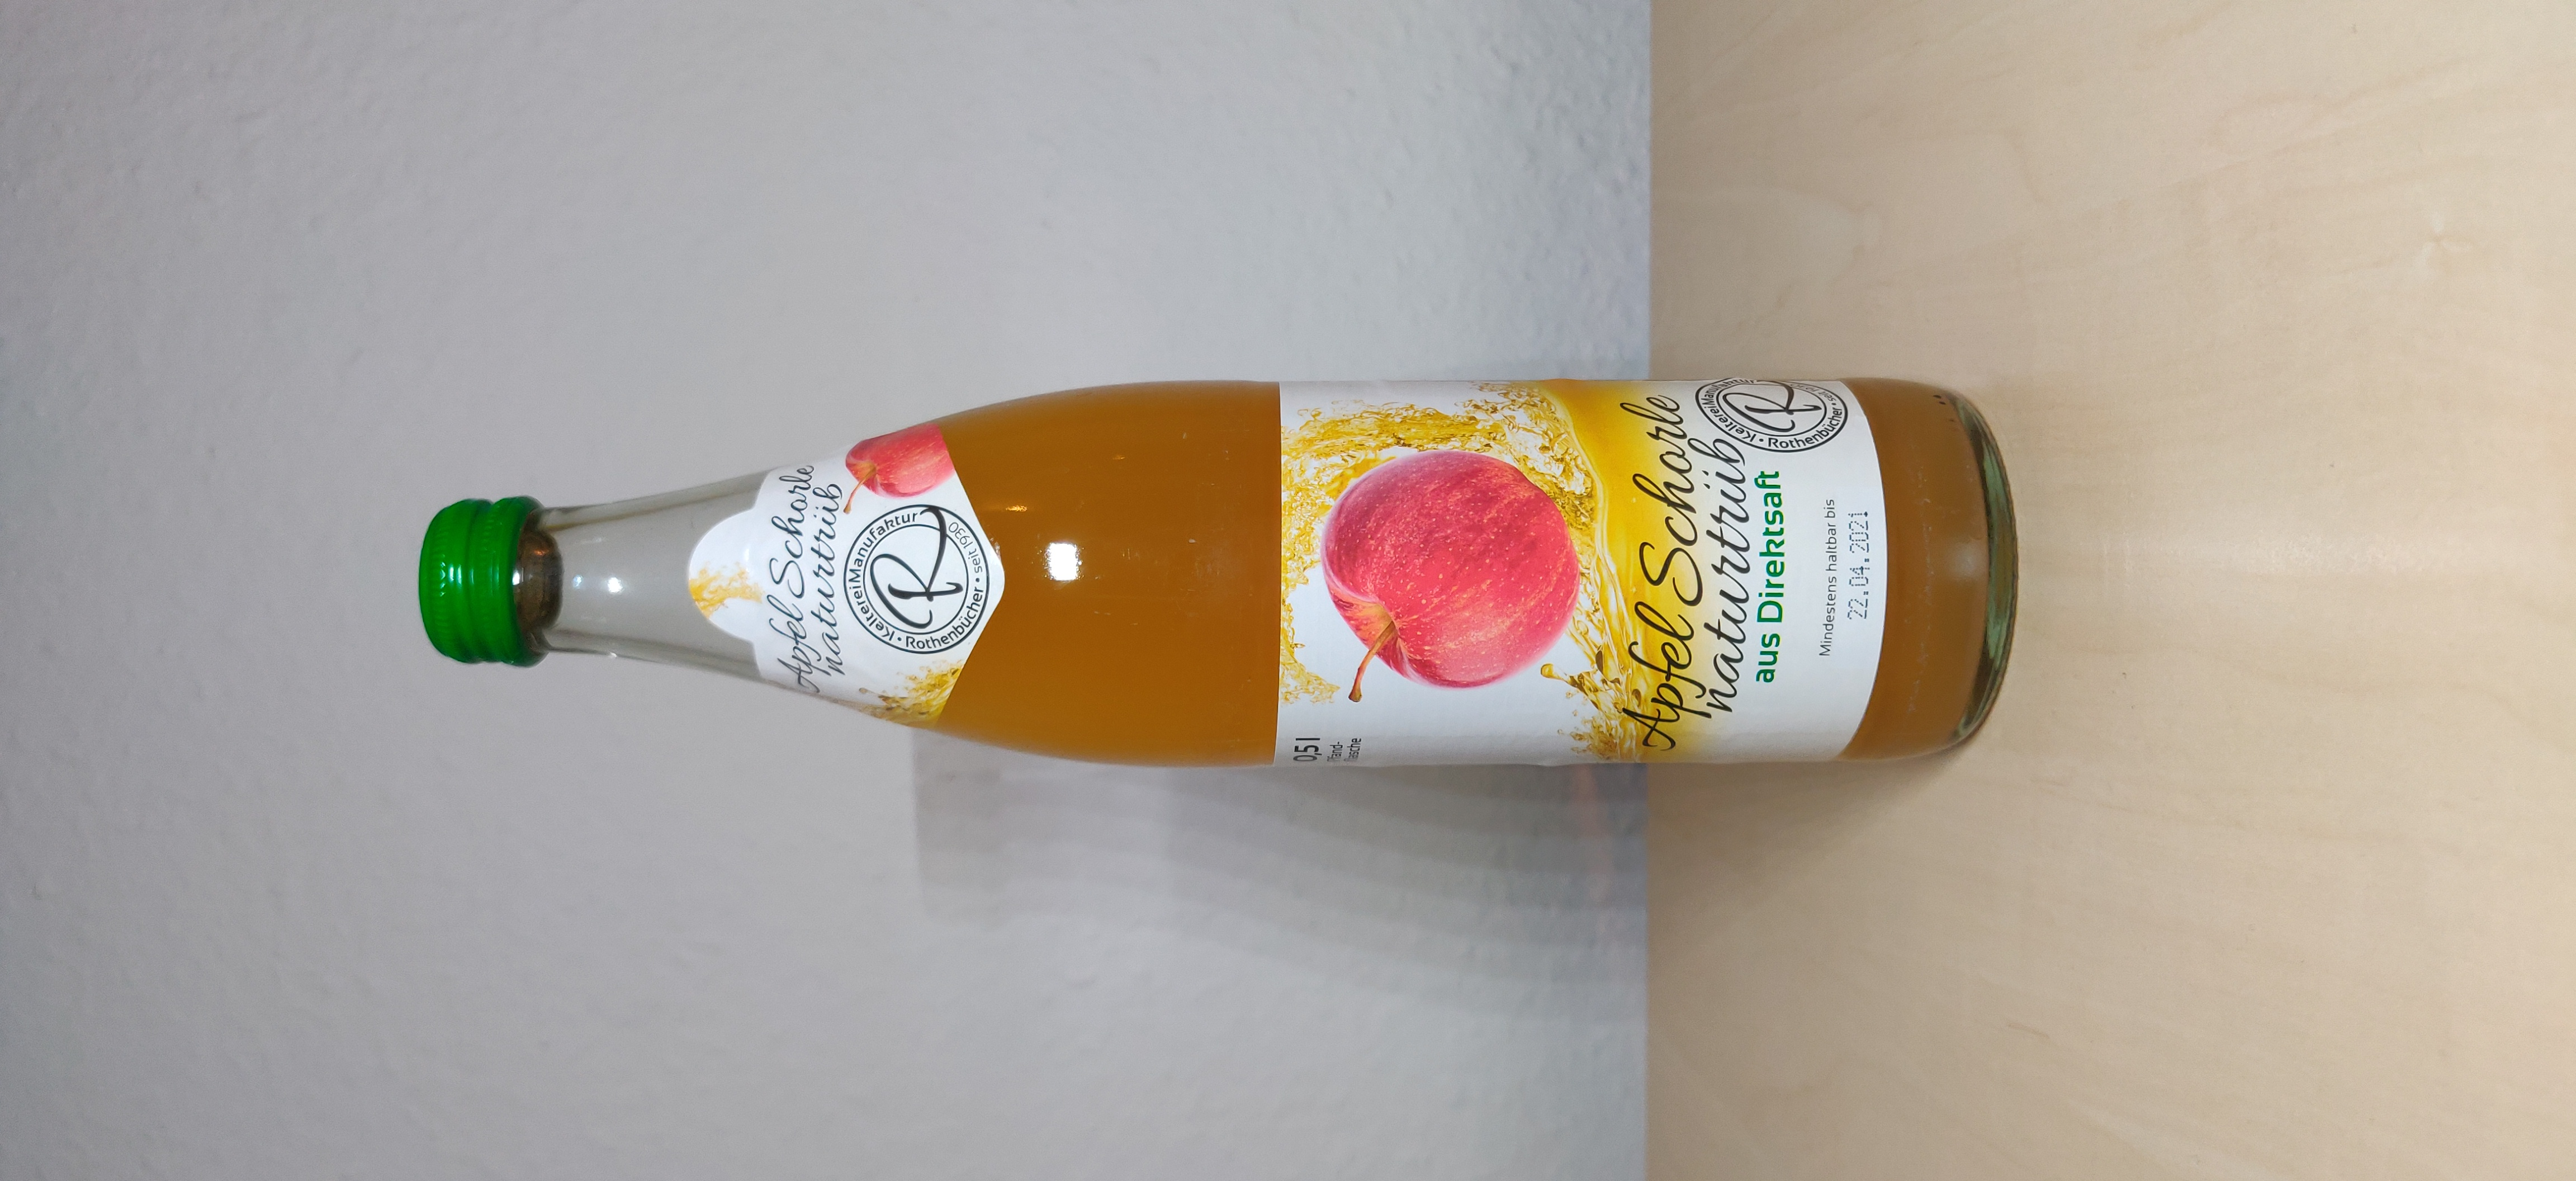
\includegraphics[width=0.30\textwidth]{Bilder/johannisbeerschorle.jpg}}\hfill
	\subfigure[Stenger Apfelsaftschorle]{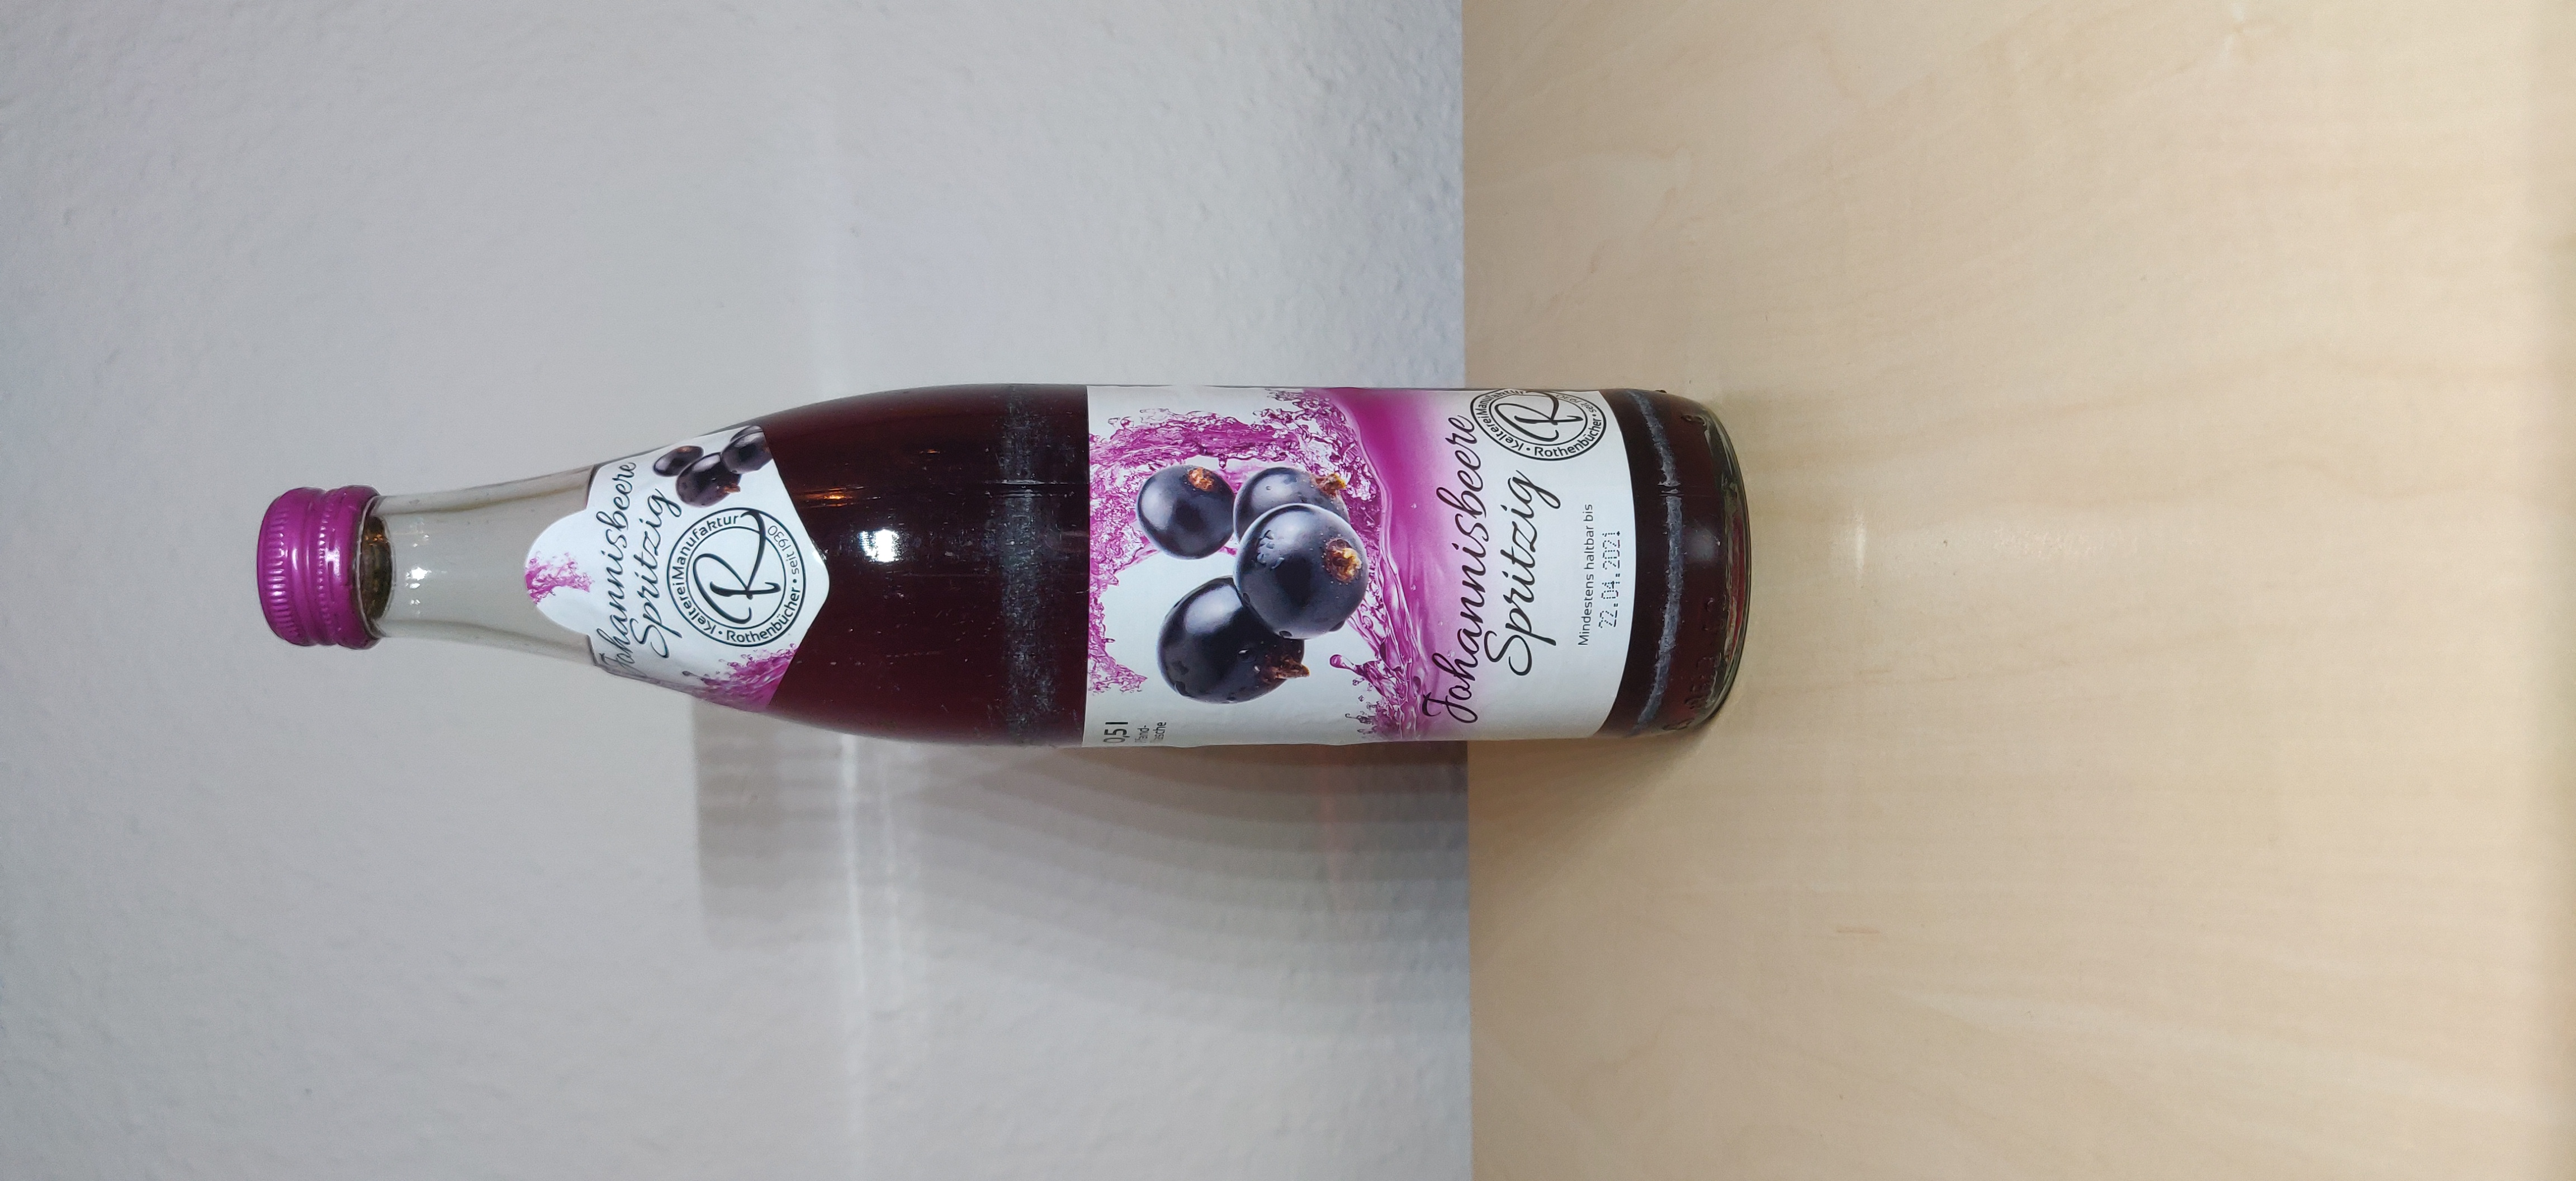
\includegraphics[width=0.30\textwidth]{Bilder/apfelsaftschorle.jpg}}\hfill
	\subfigure[Vitamalz Malzbier]{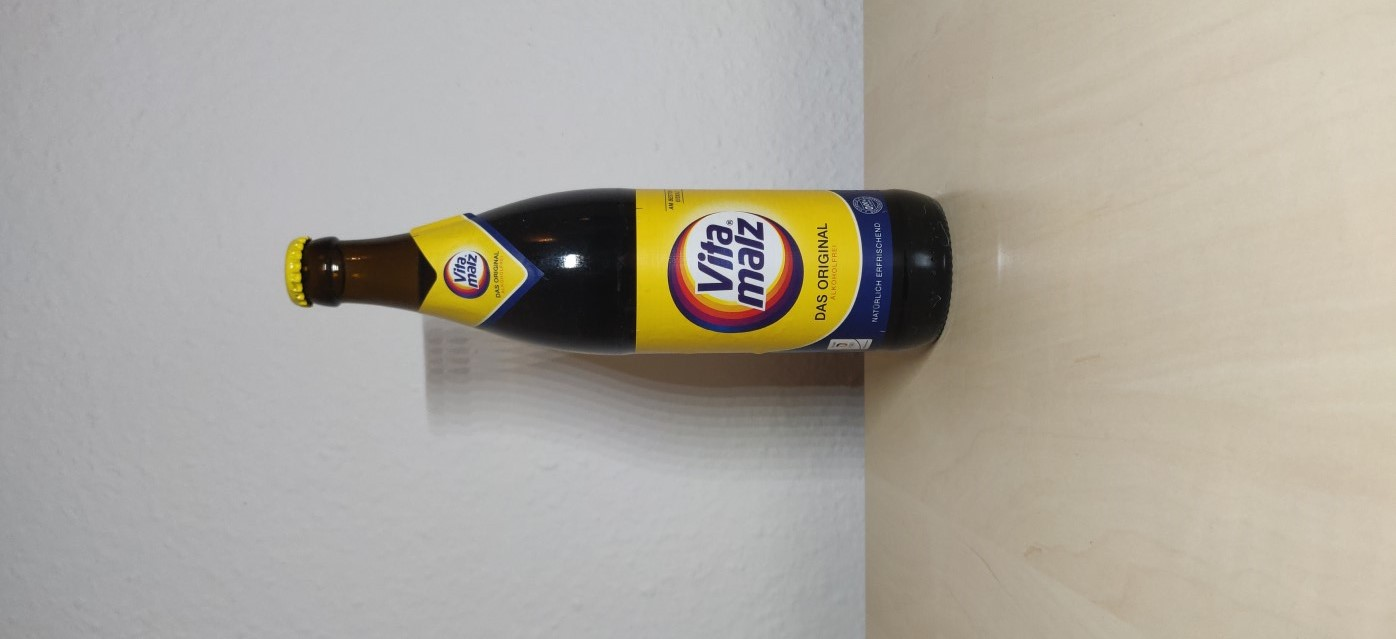
\includegraphics[width=0.30\textwidth]{Bilder/malzbier.jpg}}
	\caption{Die neun Datensatz-Kategorien}
	\label{categories}
\end{figure}

Der Datensatz ist 1.45 GB groß und besteht aus 1088 manuell annotierten Bildern. Sie dienen später dazu die ausgewählten Objektdetektoren zu trainieren. Die Bilder besitzen eine Auflösung von 2112x4608 Pixeln mit einer Farbtiefe von 24 Bit. Alle neuen Kategorien sind nahezu gleich häufig im Datensatz vorhanden. 

\begin{figure}[H]
	\begin{center}
		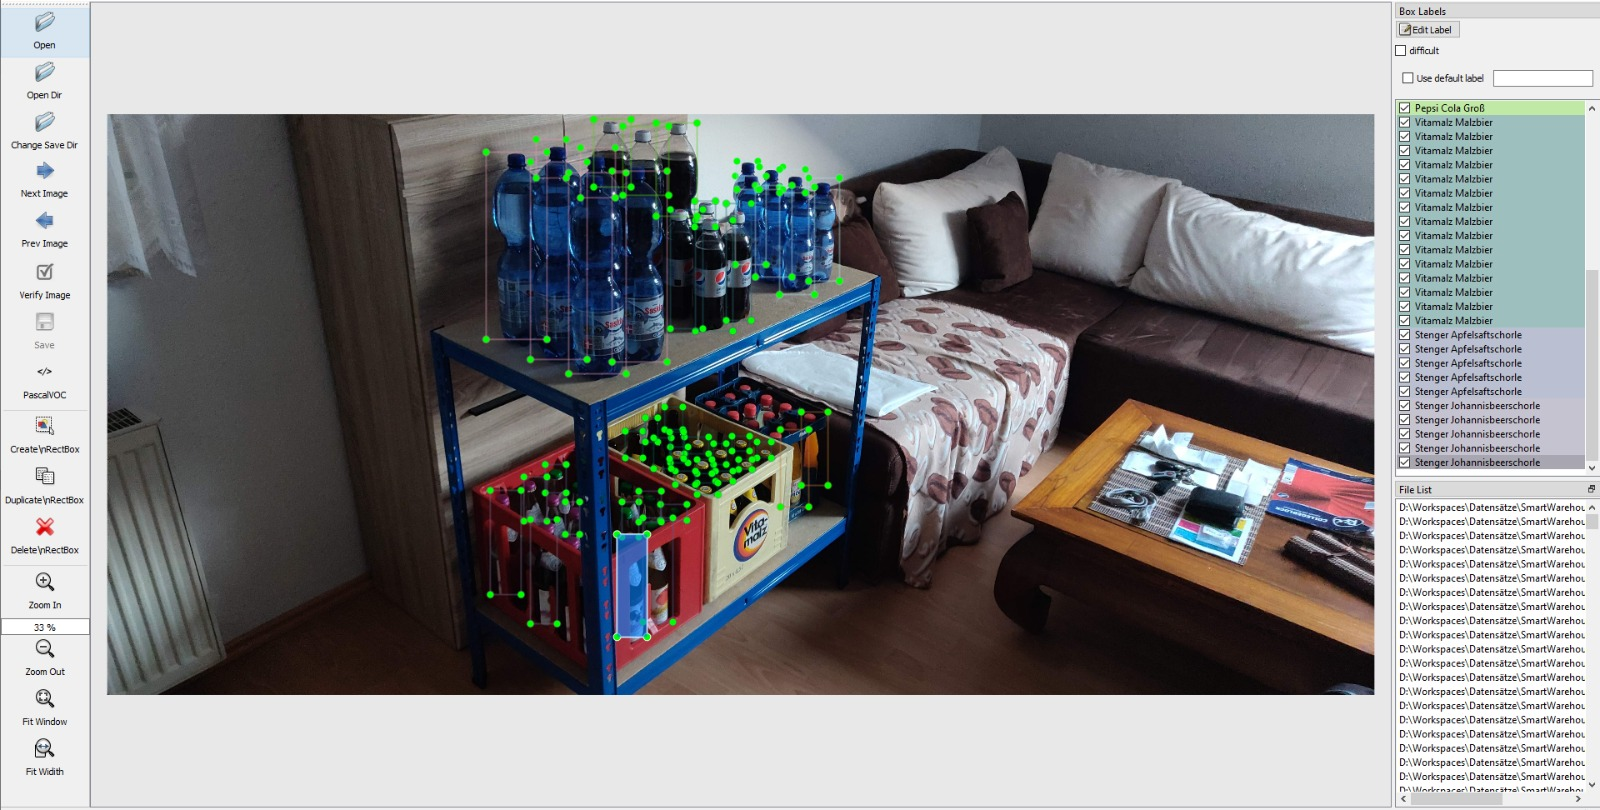
\includegraphics[width=16cm]{Bilder/labelImg.jpeg} 
		\caption[Annotieren der Bilddaten mit labelImg]{Annotieren der Bilddaten mit labelImg}
		\label{labelImg}
	\end{center}
\end{figure}

Durch das Tool \textit{LabelImg} wurden die Daten sowohl für das \textit{PascalVOC}, als auch das \textit{YOLO} Format annotiert (siehe Abbildung \ref{labelImg}). Im initialen Datensatz sind auf 75\% der Bilder die Objekte der jeweiligen Kategorien einzeln und klar erkennbar abgebildet. Hierdurch wird erhofft, dass Modell zunächst auf die Muster der jeweiligen Objekte zu trainieren. Hinsichtlich der im folgenden Kapitel eingeführten Bewertungskriterien sind weitere 12,5\% der Bilder so ausgewählt, dass ein möglichst gutes Inferenzverhalten, gerade bei schwierigen Aufnahmeumständen und möglichen Problemfällen, gewährleistet werden kann. Dies umfasst vor allem Situationen der starken Überdeckung, unterschiedlicher Entfernungen und Blicklagen sowie wechselnde Lichtverhältnisse. Je nach Umgebung wurden Bilder dieses Anteils als schwer erkennbar markiert. Auch wurde darauf geachtet, die Hintergründe der zu detektierenden Objekte kontinuierlich zu variieren. Um das Warenhaus zu simulieren, sind in den letzten 12,5\% der Bilder die Objekte auf Regalen angeordnet, jeweils hintereinander oder in Getränkekästen. Ein Ausschnitt aus dem Datensatz kann in Abbildung \ref{dataset} eingesehen werden. 

\begin{figure}[H]
	\subfigure{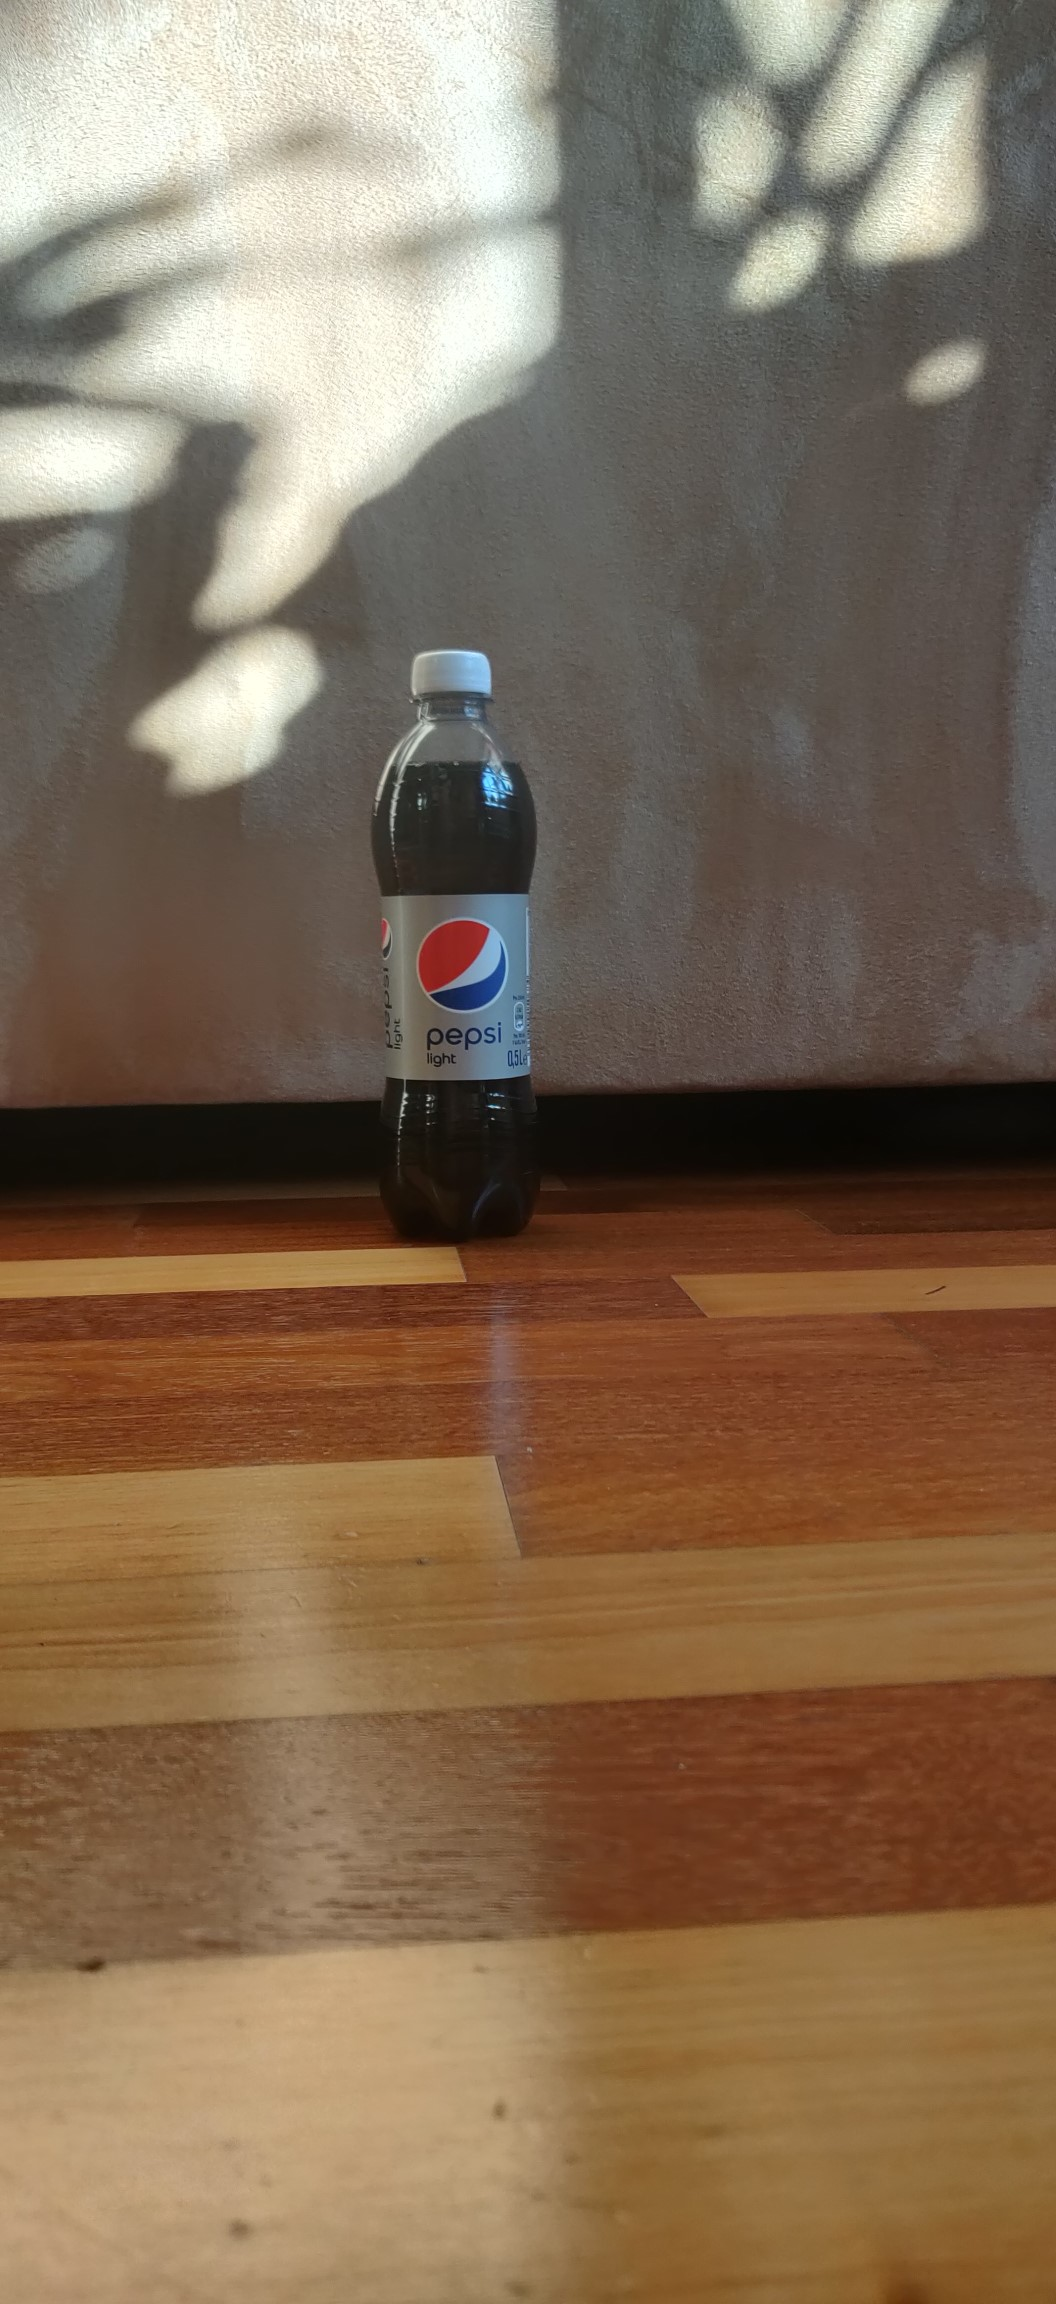
\includegraphics[width=0.20\textwidth]{Bilder/dataset1.jpg}}\hfill
	\subfigure{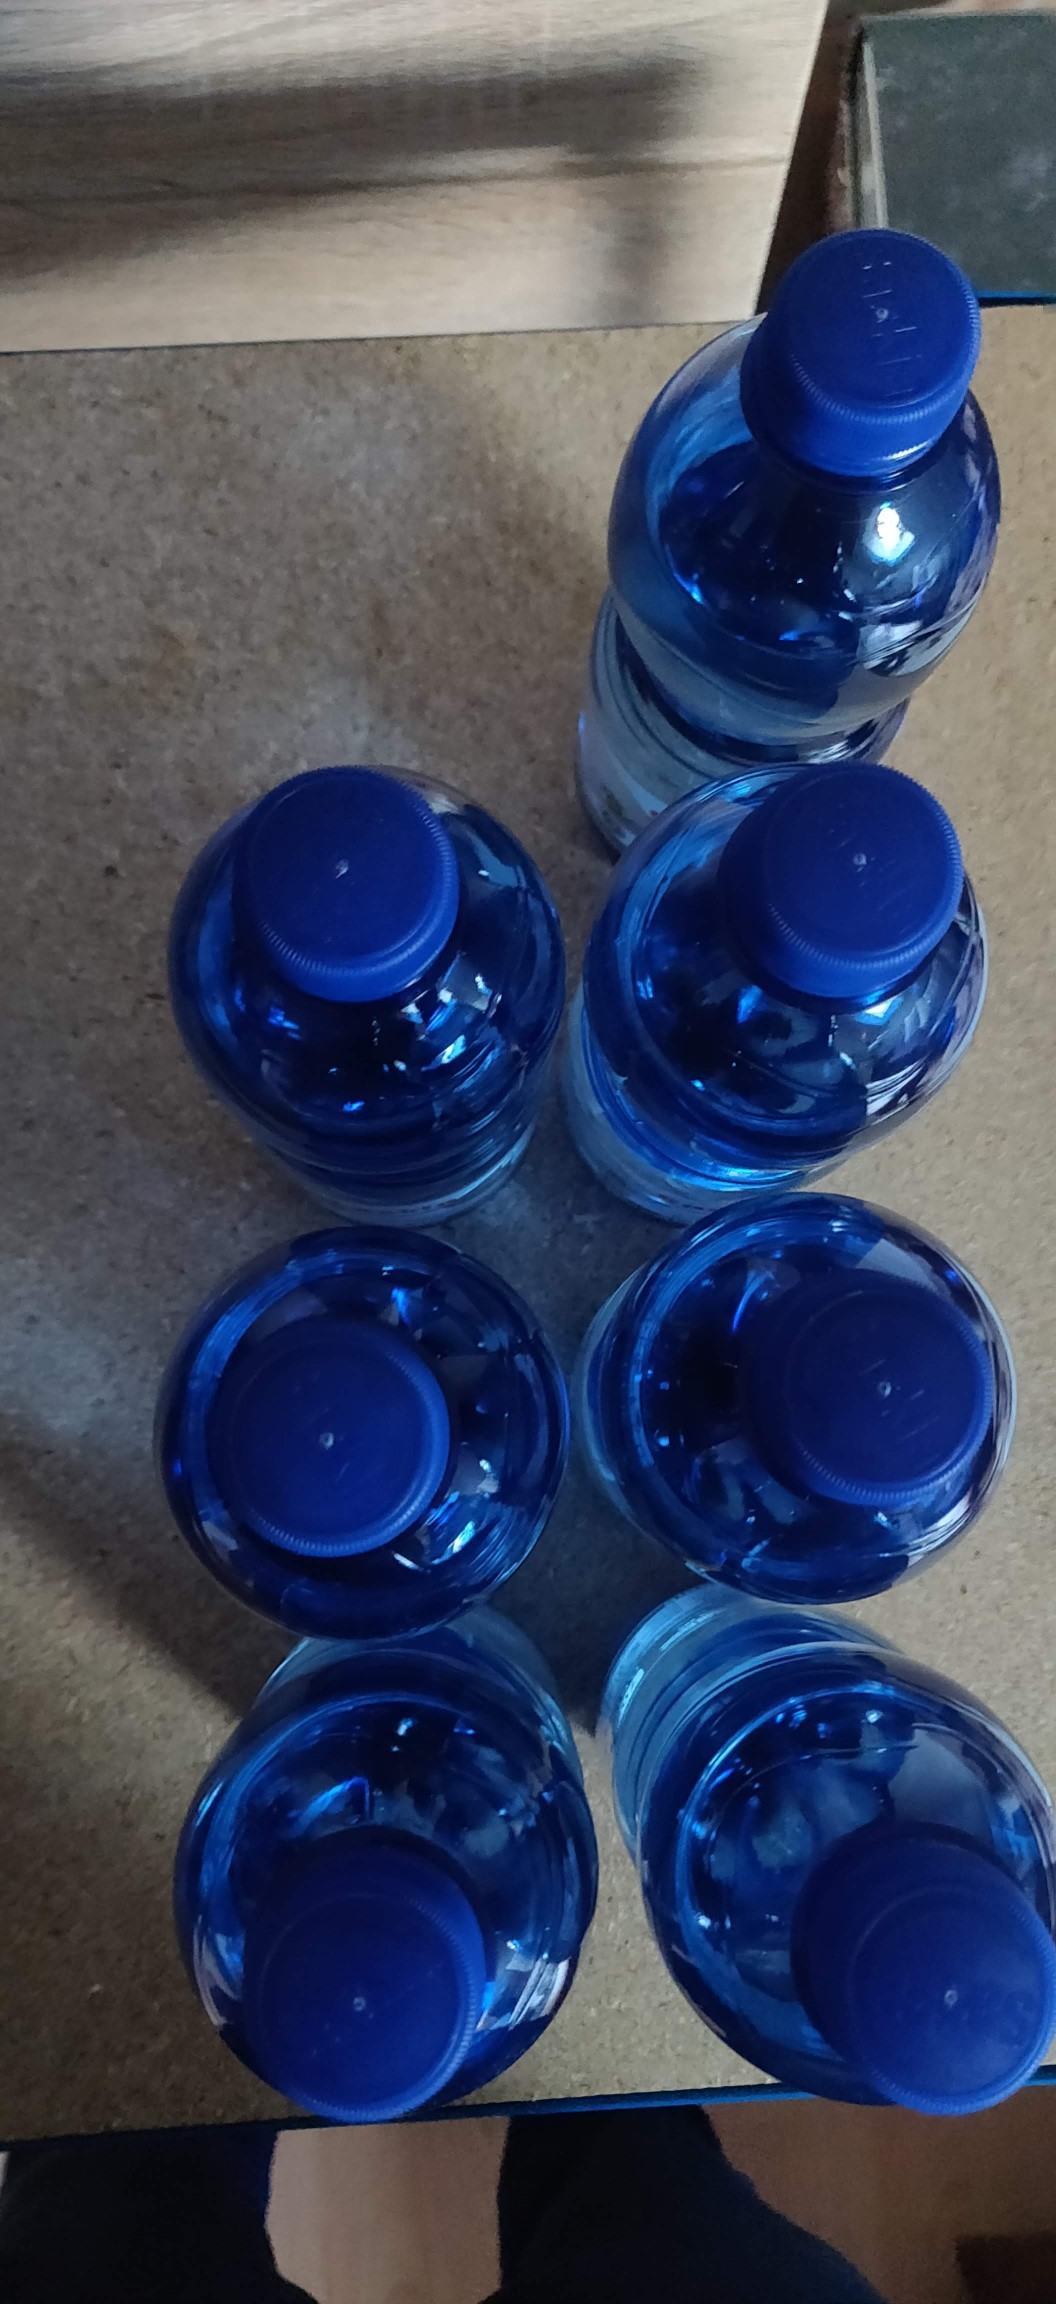
\includegraphics[width=0.20\textwidth]{Bilder/dataset2.jpg}}\hfill
	\subfigure{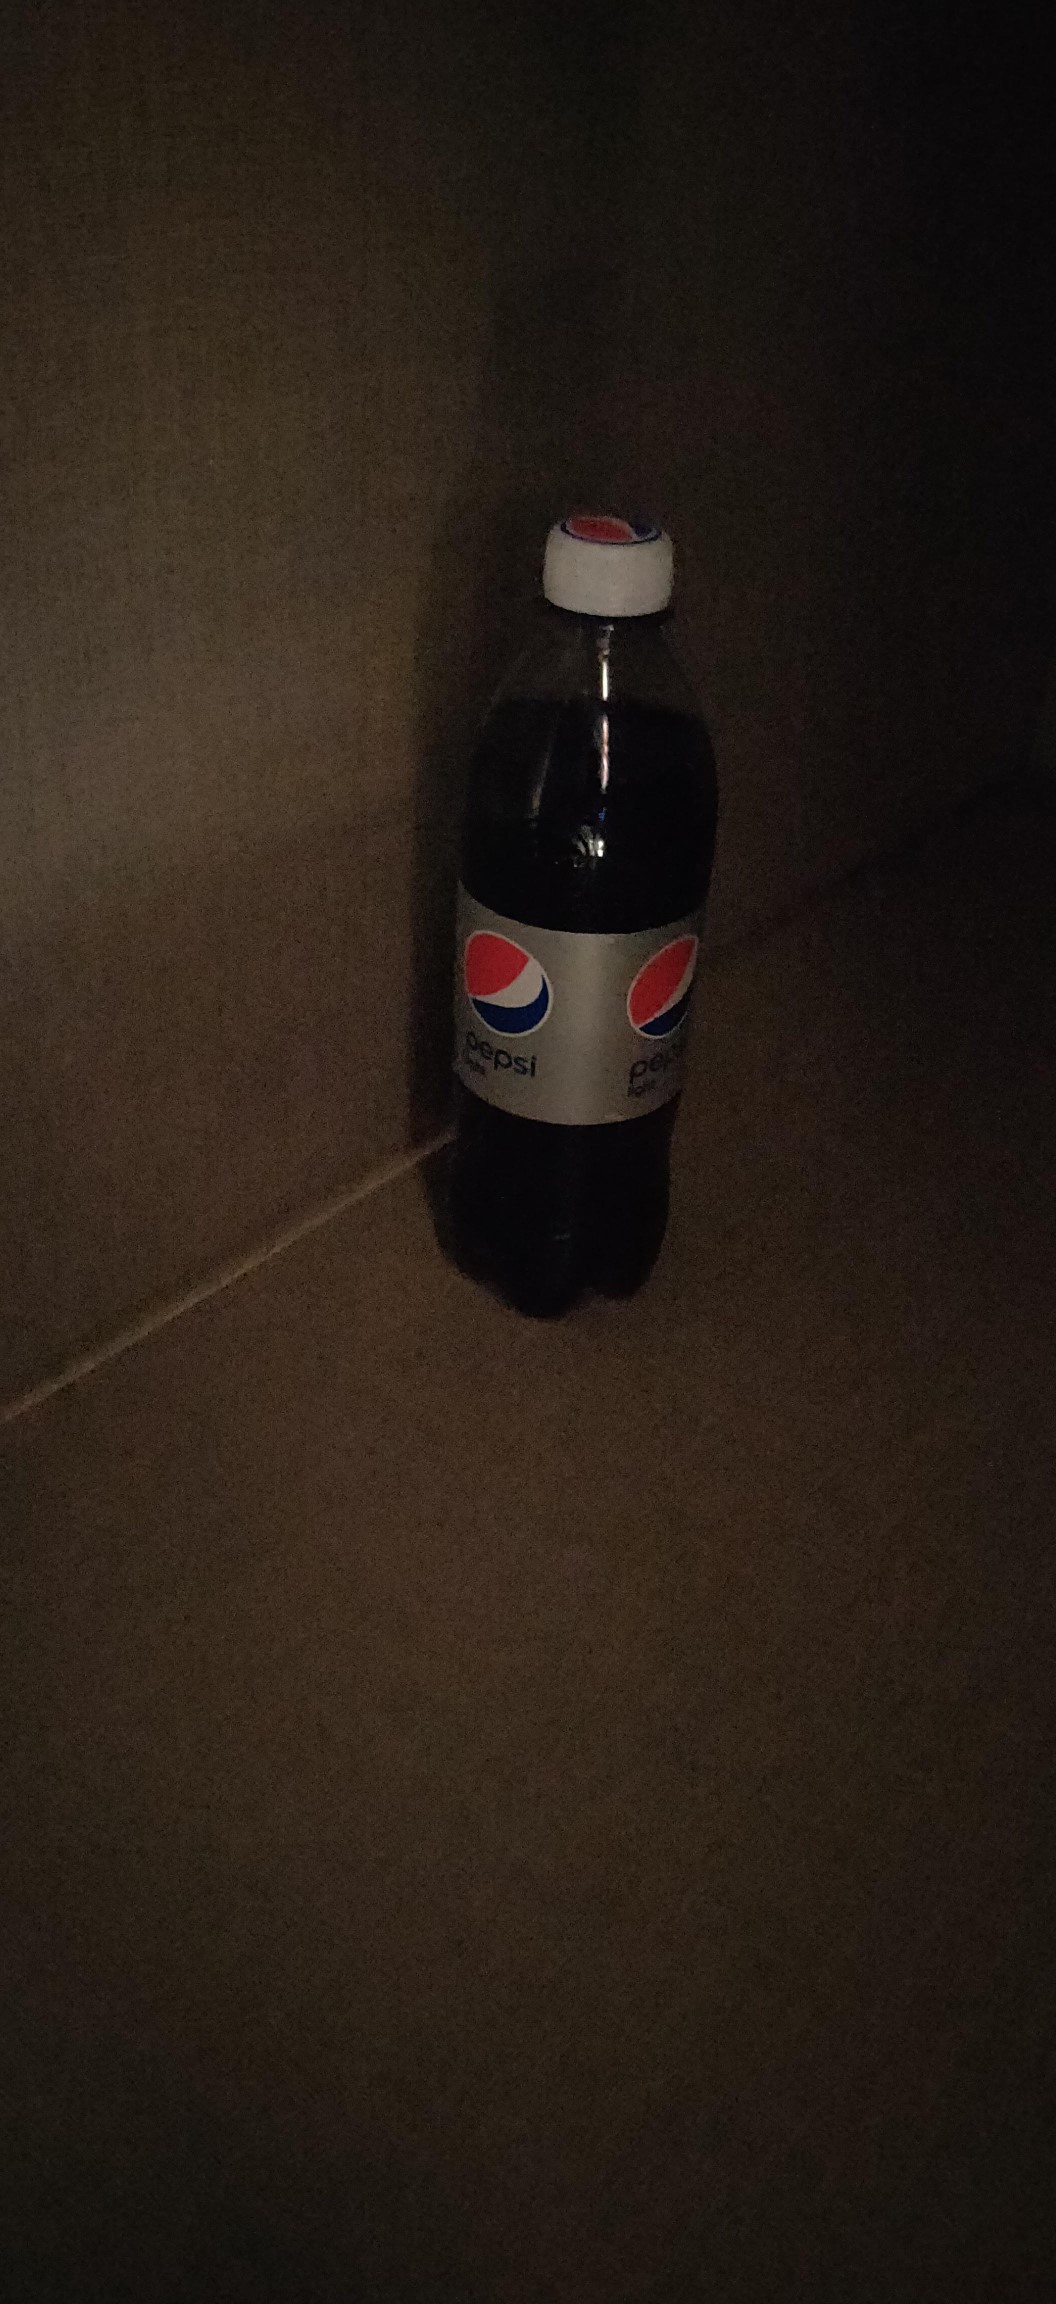
\includegraphics[width=0.20\textwidth]{Bilder/dataset3.jpg}}\hfill
	\subfigure{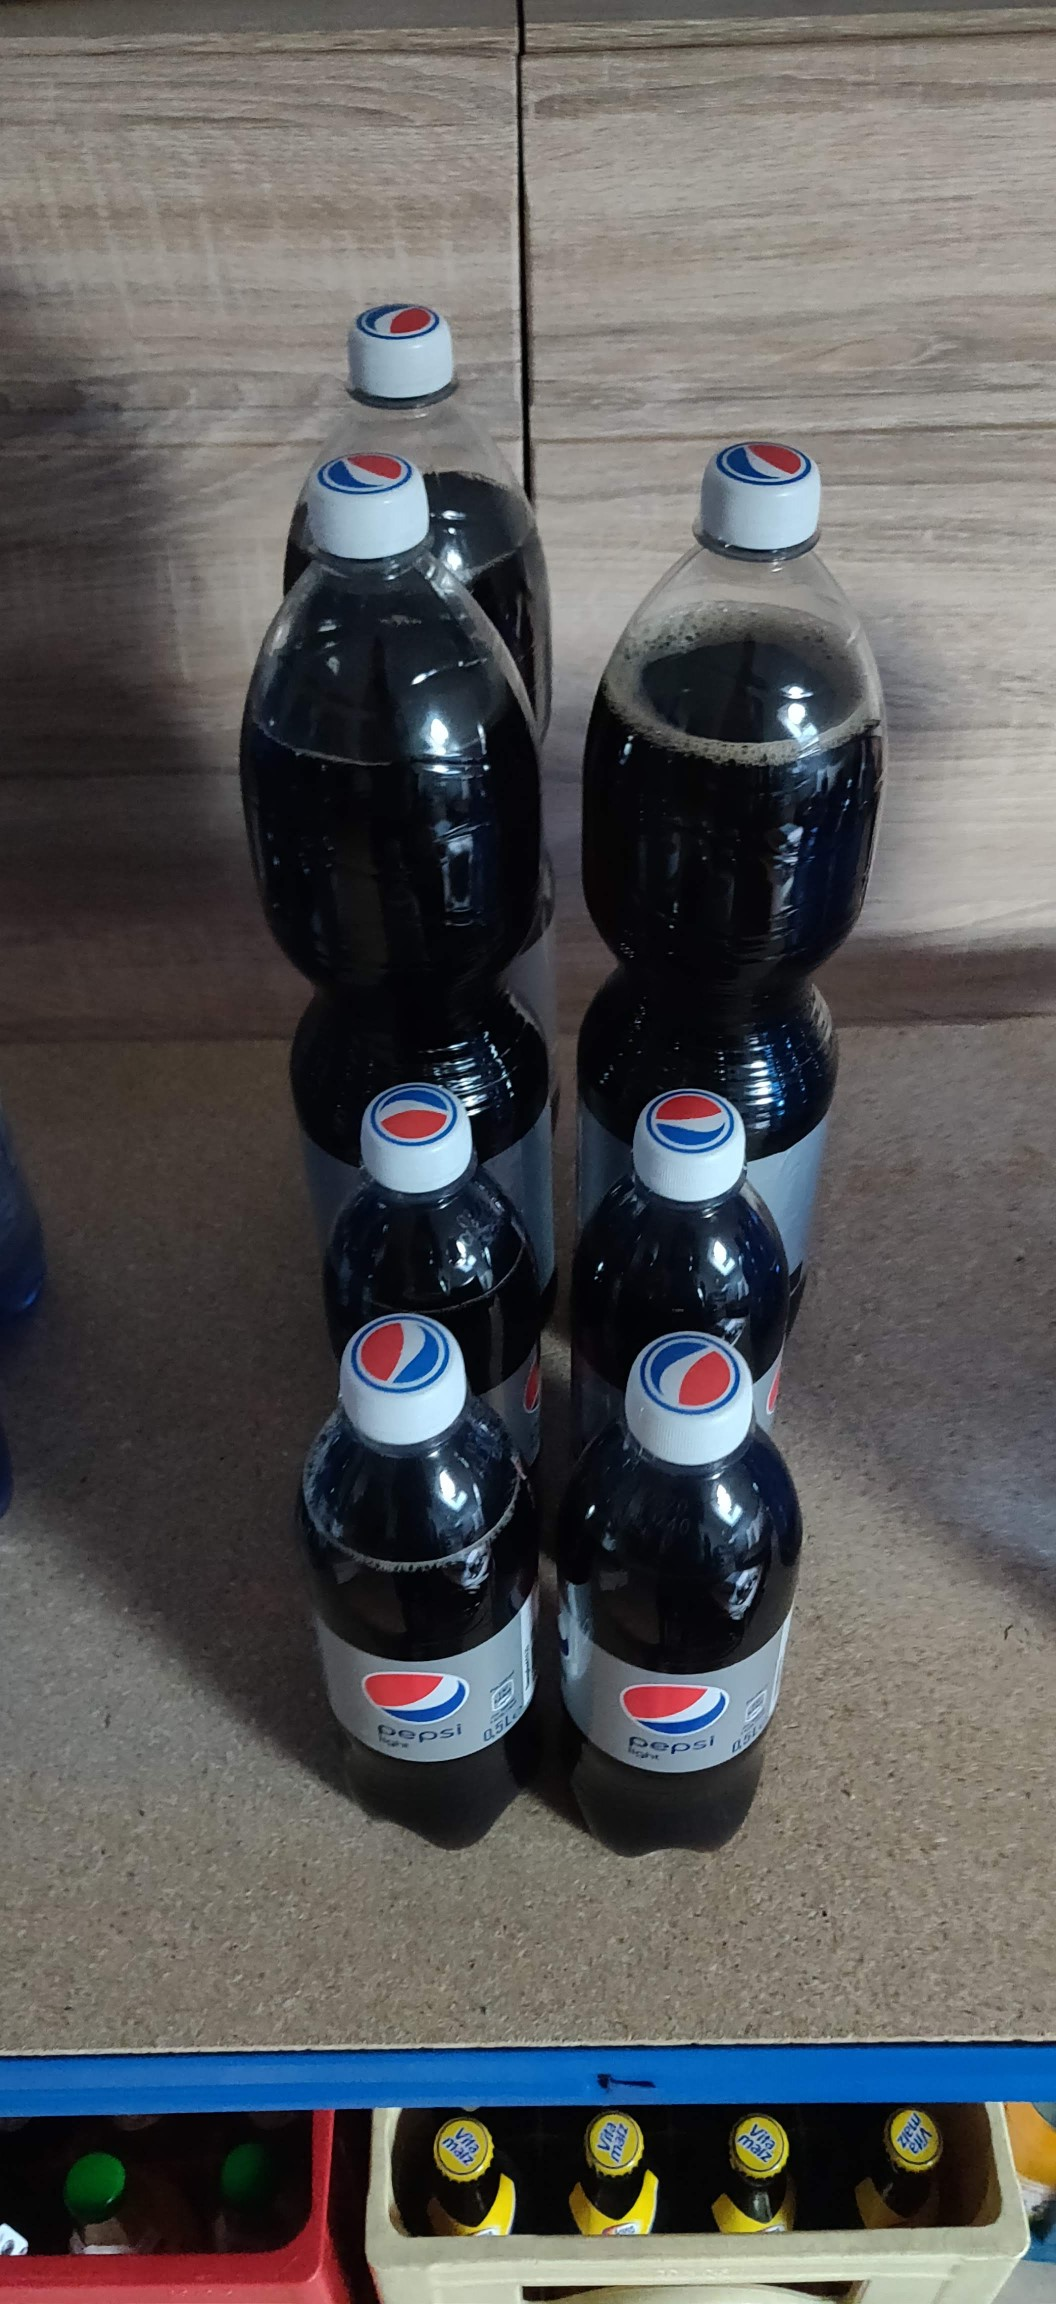
\includegraphics[width=0.20\textwidth]{Bilder/dataset4.jpg}}\hfill
	\caption{Ausschnitt aus dem SmartWarehouse Datensatz}
	\label{dataset}
\end{figure}

Aus dem Gesamtdatensatz von 1088 Bildern wurden 90 Bilder für die spätere Validierung herausgezogen. Die restlichen 998 bestehen aus 200 Bildern Testdaten und 798 Bildern für das Training. Der Datensatz wurde sowohl für das \textit{PascalVOC} Format, als auch für das \textit{YOLO} Format auf \textit{Kaggle}\footnote{Kaggle ist eine Online-Plattform für Datenwissenschaftler. Hier werden regelmäßig neue Datensätze bereitgestellt, oft im Zusammenhang mit bestimmten dazugehörigen Problemstellungen, die es unter der Gemeinschaft zu lösen gilt. Für bestimmte Problemstellungen werden sogar Preisgelder für deren Lösung ausgezahlt.} veröffentlicht \cite{FelixHausberger.20200503}.
